\section{INTRODUCTION}

This document presents the report of the first project developed for the "Sensor Networks" course.

The project is based around the study of wireless sensors design and the implementation of a use case in order to obtain data from remote sensors, applying knowledge in communication protocols and in low capabilities platforms.

The system is centered around a solution designed in a previous course (Embedded platforms and communications for \acrfullr{iot}). In the course, a solution to obtain biological data from a plant and other parameters such as the 
GPS location was designed. This solution is presented in the \autoref{fig:solutionIntro} and uses the \texttt{DISCO-L072CZ-LRWAN1} board.
\begin{figure}[H]
    \centering
    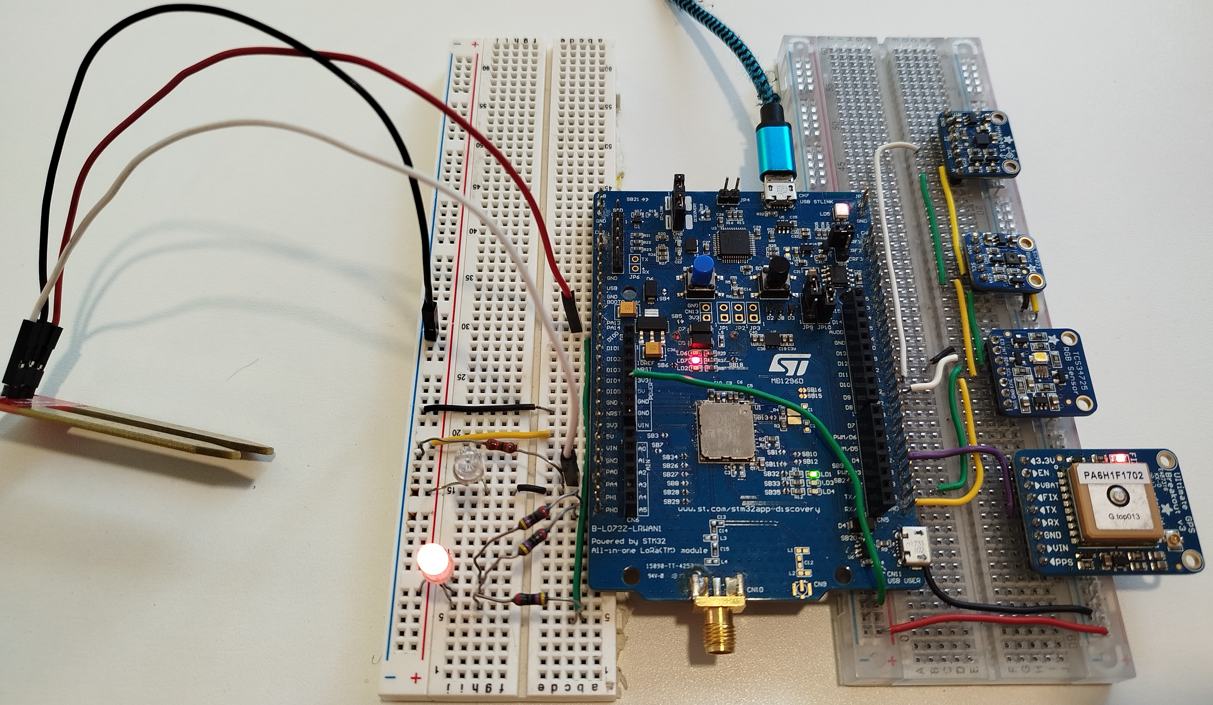
\includegraphics[width=0.53\textwidth]{images/1/sistema.png}
    \caption{Solution developed in the previous course.}
    \label{fig:solutionIntro}
\end{figure}

To further expand on this idea, the task presented is to modify the system and send the data with wireless communications to allow the final user to see all the information needed regarding the status of the plant 
remotely. To achieve this, the \acrfullr{lorawan} module of the board is used. This module combined with a event queue based solution will send the information of the plant to 
a remote gateway and routed to a network server that will process the data into a dashboard.

The final dashboard that presents the information obtained is is presented in \autoref{fig:finalDashboard}.
\begin{figure}[H]
    \centering
    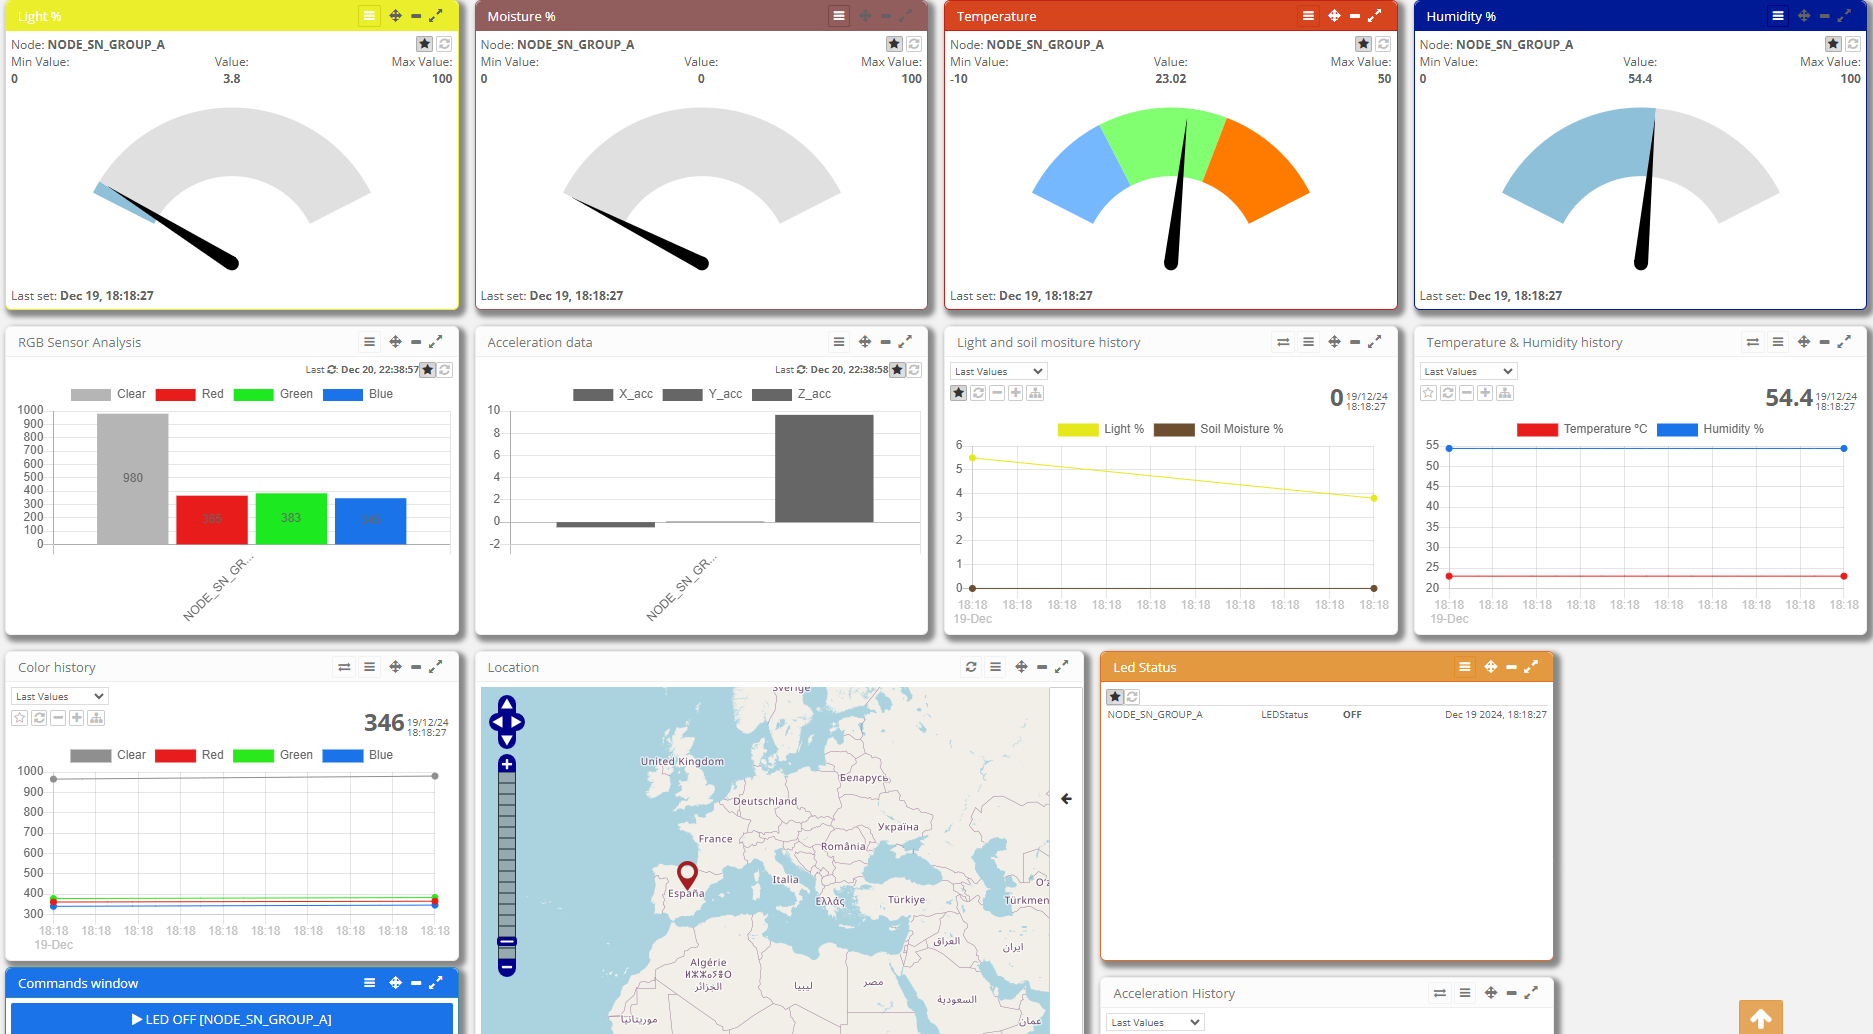
\includegraphics[width=0.8\textwidth]{images/1/FinalDashboard.png}
    \caption{Final dashboard of the system.}
    \label{fig:finalDashboard}
\end{figure}